\documentclass{ximera}

\input{../../preamble.tex}

\author{Ivo Terek}
\license{Creative Commons Attribution-ShareAlike 4.0 International License}

%\outcome{Calculating the rate of change.}
%\outcome{Discuss the meaning of antiderivatives of a position function.}

\begin{document}
\begin{exercise}

  Consider the functions $f(x) = x^2$ and $g(x) = -\frac{x^2}{4}+x-3$. Their graphics are below --- $y=f(x)$ in blue and $y=g(x)$ in red.

    \begin{image}
 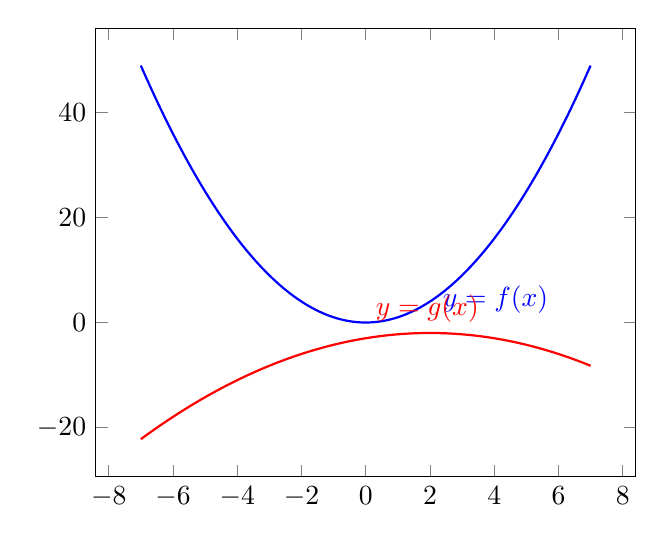
\begin{tikzpicture}
   \begin{axis}
     \addplot[samples=200,thick, domain=-7:7, color=blue]{x^2} node[pos=0.55,right]{\text{$y=f(x)$}};
     \addplot[samples=200,thick,domain=-7:7, color=red]{-(x^2)/4 + x-3} node[pos=0.73,above]{\text{$y=g(x)$}};
   \end{axis}
 \end{tikzpicture}
 \end{image}


 To produce the graph of $g$ in terms of the graph of $f$, in which order should you perform the following steps? Enter the numbers 1, 2, 3, and 4, accordingly.

 {\bf Hint:} Finding the concrete relation $g(x) = af(bx-c)+d$ might be helpful.

  \begin{itemize}
  \item Horizontal shift right 1 unit. $\answer{3}$
  \item Vertical shift up 2 units. $\answer{1}$
  \item Reflection across the $x$-axis. $\answer{2}$
  \item Horizontal stretching by a factor of $2$. $\answer{4}$.
  \end{itemize}

\end{exercise}
\end{document}
